\documentclass{beamer}
\setbeamertemplate{navigation symbols}{}
\usepackage[T1]{fontenc}
\usepackage[utf8]{inputenc}
\usepackage{tabularx}
\usepackage{subscript}
\usepackage{graphicx}


\usetheme{Montpellier}
\beamersetuncovermixins{\opaqueness<1>{25}}{\opaqueness<2->{15}}
\begin{document}
\title{Hydroelectricity}
\author{Luca Hülsmann \and Luca Kiebel}
\date{\today}

\begin{frame}
\titlepage
\end{frame}

\begin{frame}
\frametitle{Table of Contents}\tableofcontents
\end{frame}

\section{Are there different ways to produce energy from the same source?}
\begin{frame}
\frametitle{Are there different ways to produce energy from the same source?}
\begin{itemize}
	\item Dams
	\item Tide
	\item Pumped-Storage
	\item Run-of-the-river
\end{itemize}
\end{frame}

\section{How does Hydroelectricity work?}

%Hülsmann
\subsubsection{Dams}
\begin{frame}
\frametitle{How do dams work?}
	\begin{itemize}
		\item Water flows through turbines
		\item Potential energy of the water proportional to distance from turbine
		\item Turbines power generators
	\end{itemize}
\end{frame}

\begin{frame}
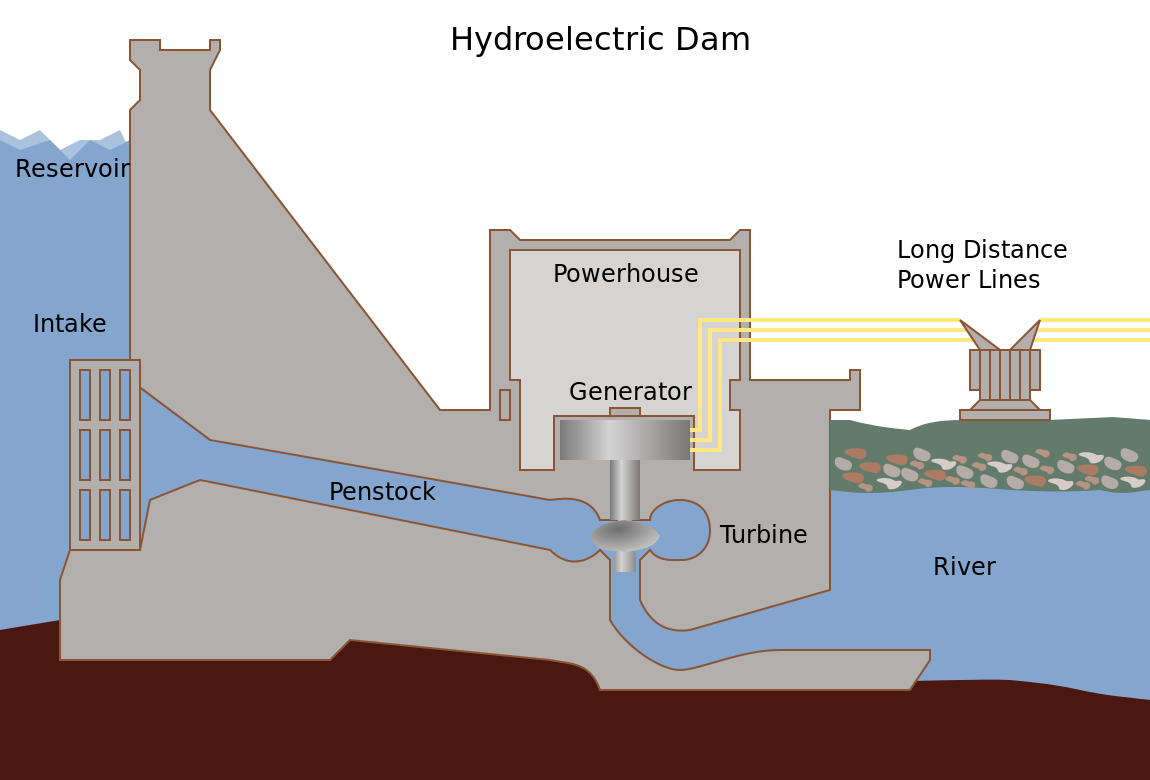
\includegraphics[width=0.9\textwidth]{dam}
\end{frame}

%Kiebel
\subsubsection{Tidal}
\begin{frame}
\frametitle{How does Tidal power generation work?}
\begin{itemize}
	\item Tides power windmill-like water wheels
	\item Highly predictable
\end{itemize}
\end{frame}

%Hülsmann
\section{Where is it used?}
\begin{frame}
\frametitle{Where is it used?}
\begin{itemize}
	\item Everywhere in the world
	\item China produces 1064 TWh (18.7\%)
	\item Norway produces 129 TWh (96.0\%)
\end{itemize}
\end{frame}

\begin{frame}
\frametitle{Usage around the world}
    \begin{tabularx}{\textwidth}{X|XX}
    Country & Ann. prod. (TWh) & \% of total prod.\\ \hline
    China   & 1064                                  & 18.7                   \\
    Canada  & 383                                   & 58.3                   \\
    Brasil  & 373                                   & 63.2                   \\
    US      & 282                                   & 6.5                    \\
    Russia  & 177                                   & 16.7                   \\
    India   & 132                                   & 10.2                   \\
    Norway  & 129                                   & 96.0                   \\
\end{tabularx}
\end{frame}

%Kiebel
\section{Efficiency}
\begin{frame}
\frametitle{How efficient is it?}
	Large modern water turbines operate at mechanical efficiencies greater than 90\%
\end{frame}

%Hülsmann
\section{Sustainability}
\begin{frame}
\frametitle{How sustainable is it?}
As long as there is water on the planet and it's flowing somewhere you can build water power plants. Thus it's pretty sustainable.
\end{frame}

%Kiebel
\section{Downsides}
\begin{frame}
\frametitle{Disatvantages}
\begin{itemize}
	\item Ecosystem damage and loss of land
	\item Water loss by evaporation
	\item Siltation and flow shortage
	\item Relocation
	\item Failure risks
\end{itemize}
\end{frame}

%Hülsmann
\section{Benefits}
\begin{frame}
\frametitle{Advantages}
\begin{itemize}
	\item Flexibility
	\item Low cost
	\item Reduced CO\textsubscript{2} emissions
\end{itemize}
\end{frame}

\section{Sources}
\begin{frame}
\frametitle{Sources}
\begin{itemize}
	\item https://en.wikipedia.org/wiki/Norway, accessed November 18, 2017
	\item https://en.wikipedia.org/wiki/Hydroelectricity, accessed November 18, 2017
	\item https://en.wikipedia.org/wiki/Water\_turbine, accessed November 18, 2017
\end{itemize}

\end{frame}

\end{document}
